% Asset ID: FAS2DiscreteRandomVariablesTikZ-002
% Source: Transcript coding section + CCEA FAS2-DIST-LO006
% Related lesson section: #8 Core Theory, #9 Visual Asset Integration, #15 Exam Technique Notes
% Used placeholder: FAS2DiscreteRandomVariablesTikZ-002
% Purpose: Visualise linear coding Y=aX+b for expected value and variance.

\documentclass[tikz,border=8pt]{standalone}
\usepackage{amsmath}
\usepackage{xcolor}
\usetikzlibrary{arrows.meta,positioning,calc}
\definecolor{Canvas}{HTML}{FAF9F6}
\definecolor{Ivory}{HTML}{FFFFF0}
\definecolor{Line}{HTML}{E5E5EA}
\definecolor{Gold}{HTML}{C5A059}
\definecolor{SoftPink}{HTML}{FBEFEF}
\definecolor{Text}{HTML}{2C2C2E}
\begin{document}
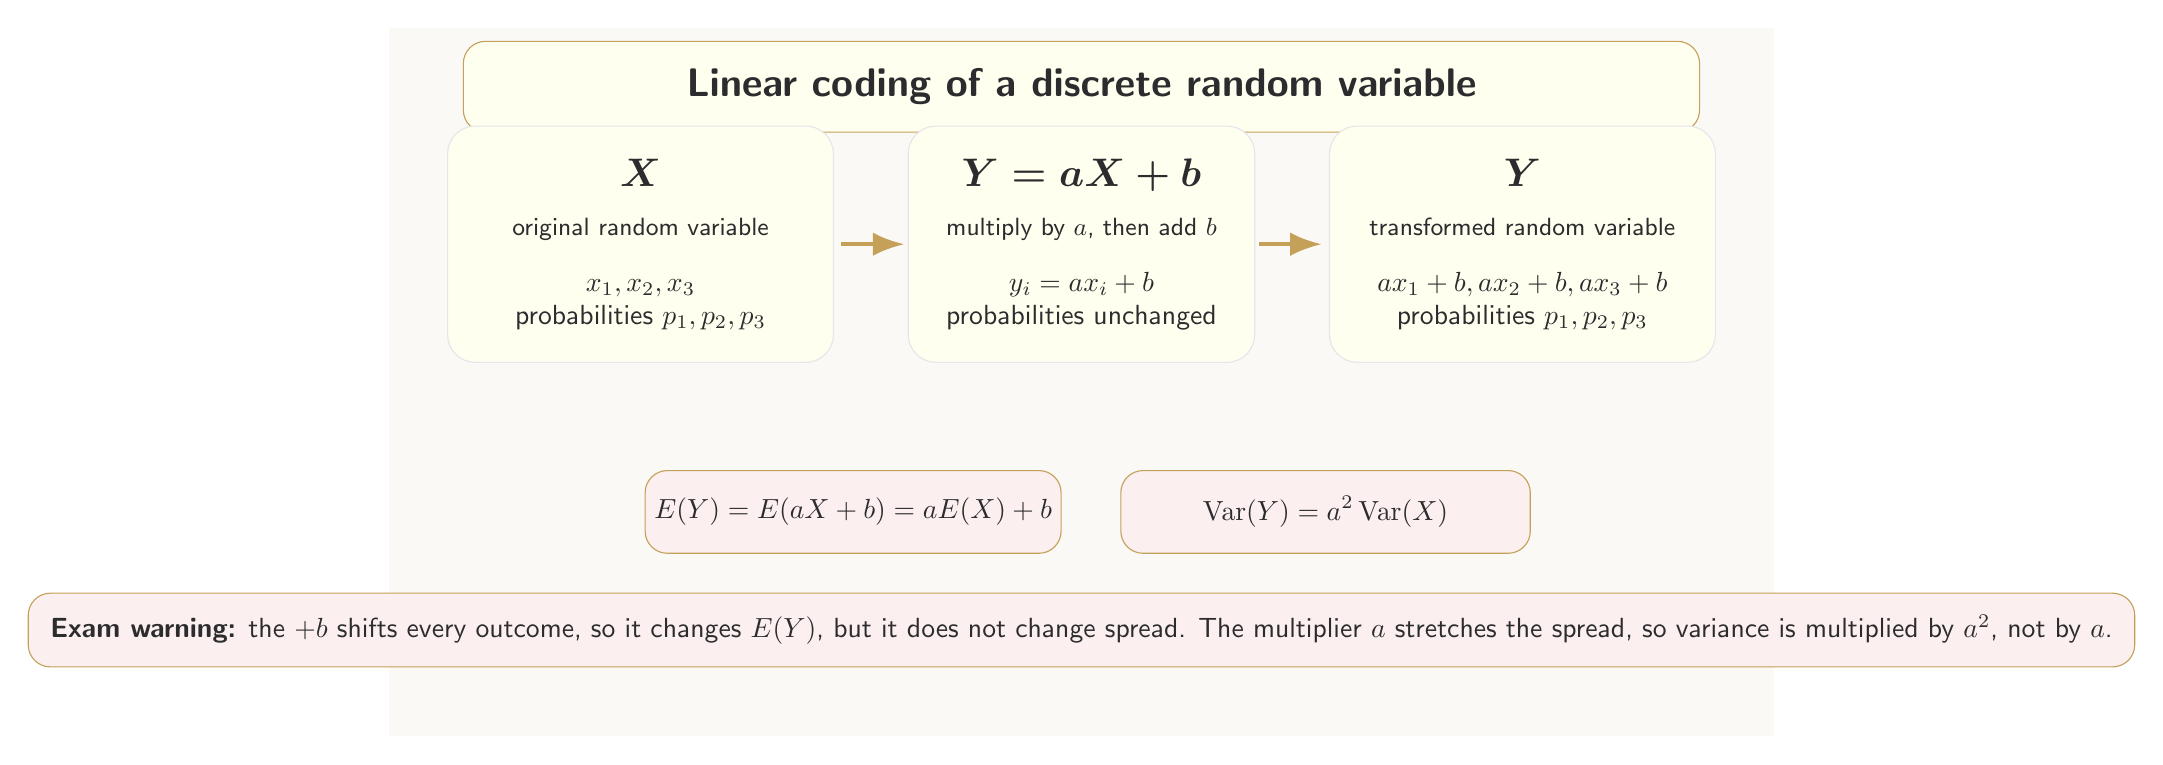
\begin{tikzpicture}[font=\sffamily,every node/.style={text=Text},bigbox/.style={rounded corners=10pt,draw=Line,fill=Ivory,minimum width=4.9cm,minimum height=3.0cm,align=center},formula/.style={rounded corners=8pt,draw=Gold,fill=SoftPink,minimum width=5.2cm,minimum height=1.05cm,align=center,font=\sffamily\bfseries},arrowstyle/.style={-{Latex[length=4mm,width=3mm]},line width=1.4pt,draw=Gold}]
\fill[Canvas] (-1,-5.9) rectangle (16.6,3.1);
\node[draw=Gold,rounded corners=8pt,fill=Ivory,minimum width=15.7cm,inner sep=10pt] at (7.8,2.35) {\Large \textbf{Linear coding of a discrete random variable}};
\node[bigbox] (Xbox) at (2.2,0.35) {\Large $\boldsymbol{X}$\\[6pt]\small original random variable\\[8pt] $x_1,x_2,x_3$\\ probabilities $p_1,p_2,p_3$};
\node[bigbox,minimum width=4.4cm] (Trans) at (7.8,0.35) {\Large $\boldsymbol{Y=aX+b}$\\[6pt]\small multiply by $a$, then add $b$\\[8pt] $y_i=ax_i+b$\\ probabilities unchanged};
\node[bigbox] (Ybox) at (13.4,0.35) {\Large $\boldsymbol{Y}$\\[6pt]\small transformed random variable\\[8pt] $ax_1+b,ax_2+b,ax_3+b$\\ probabilities $p_1,p_2,p_3$};
\draw[arrowstyle] (4.75,0.35) -- (5.55,0.35);
\draw[arrowstyle] (10.05,0.35) -- (10.85,0.35);
\node[formula] at (4.9,-3.05) {$\displaystyle E(Y)=E(aX+b)=aE(X)+b$};
\node[formula] at (10.9,-3.05) {$\displaystyle \operatorname{Var}(Y)=a^2\operatorname{Var}(X)$};
\node[draw=Gold,rounded corners=8pt,fill=SoftPink,inner sep=8pt,minimum width=13.8cm,align=left] at (7.8,-4.55) {\textbf{Exam warning:} the $+b$ shifts every outcome, so it changes $E(Y)$, but it does not change spread. The multiplier $a$ stretches the spread, so variance is multiplied by $a^2$, not by $a$.};
\end{tikzpicture}
\end{document}
